%%%%%%%%%%%%%%%%%%%%%%%%%%%%%%%%%%%%%%%%%%%%%%%%%%%%%%%%%%%%%%%%%%
%%%%%%%% ICML 2015 EXAMPLE LATEX SUBMISSION FILE %%%%%%%%%%%%%%%%%
%%%%%%%%%%%%%%%%%%%%%%%%%%%%%%%%%%%%%%%%%%%%%%%%%%%%%%%%%%%%%%%%%%

% Use the following line _only_ if you're still using LaTeX 2.09.
%\documentstyle[icml2015,epsf,natbib]{article}
% If you rely on Latex2e packages, like most moden people use this:
\documentclass[10pt]{article}

% use Times
\usepackage{times}
% For figures
\usepackage{graphicx} % more modern
%\usepackage{epsfig} % less modern
\usepackage{subfigure} 

% For citations
\usepackage{natbib}

% For algorithms
\usepackage{algorithm}
\usepackage{algorithmic}
\usepackage{bm}
\usepackage{amssymb,amsmath}


% As of 2011, we use the hyperref package to produce hyperlinks in the
% resulting PDF.  If this breaks your system, please commend out the
% following usepackage line and replace \usepackage{icml2015} with
% \usepackage[nohyperref]{icml2015} above.
\usepackage{hyperref}

% Packages hyperref and algorithmic misbehave sometimes.  We can fix
% this with the following command.
\newcommand{\theHalgorithm}{\arabic{algorithm}}

% Employ the following version of the ``usepackage'' statement for
% submitting the draft version of the paper for review.  This will set
% the note in the first column to ``Under review.  Do not distribute.''
\usepackage{icml2015}
\usepackage{amsmath}
\usepackage{amsmath}
\usepackage{amsfonts}
\usepackage{amssymb}

\usepackage{todonotes}

\usepackage{amsbsy}

% Employ this version of the ``usepackage'' statement after the paper has
% been accepted, when creating the final version.  This will set the
% note in the first column to ``Proceedings of the...''
%\usepackage[accepted]{icml2015}


% The \icmltitle you define below is probably too long as a header.
% Therefore, a short form for the running title is supplied here:

% Saving space by deleting running title (does this actually save space?)
%\icmltitlerunning{Submission and Formatting Instructions for ICML 2015}

\begin{document} 

\twocolumn[

% Saving space by deleting title
%\icmltitle{Submission and Formatting Instructions for \\ 
%           International Conference on Machine Learning (ICML 2015)}

% It is OKAY to include author information, even for blind
% submissions: the style file will automatically remove it for you
% unless you've provided the [accepted] option to the icml2015
% package.
\icmlauthor{Your Name}{email@yourdomain.edu}
\icmladdress{Your Fantastic Institute,
            314159 Pi St., Palo Alto, CA 94306 USA}
\icmlauthor{Your CoAuthor's Name}{email@coauthordomain.edu}
\icmladdress{Their Fantastic Institute,
            27182 Exp St., Toronto, ON M6H 2T1 CANADA}

% You may provide any keywords that you 
% find helpful for describing your paper; these are used to populate 
% the "keywords" metadata in the PDF but will not be shown in the document
\icmlkeywords{6.867, machine learning}

\vskip 0.3in
]

% Saving space by deleting abstract
%\begin{abstract} 
%The purpose of this document is to provide both the basic paper template and
%submission guidelines.
%\end{abstract} 

\section{Implement Gradient Descent}
A general-purpose gradient descent Python library was created which provides for specification of $x_0$ (the initial guess), $\eta$ (the step size), and $\epsilon$ (the convergence threshold: if two consecutive steps differ by less than this value, the algorithm terminates).  The gradient descent procedure was tested on two functions with well-known optimal values: (i)  a non-convex polynomial $f(x)$, and (ii) a negative bivariate Gaussian $p(x)$:
$$f(x) = x^4 - x^3 -x^2$$
$$p(\mathbf{x}) = \frac{-100}{2\pi|\mathbf{\Sigma}|^{1/2}}\exp{\bigg(-\frac{1}{2} (\mathbf{x} - \boldsymbol{\mu})^T\mathbf{\Sigma}^{-1} (\mathbf{x} - \boldsymbol{\mu}) \bigg)}$$

\begin{figure*}[!ht]
\centering
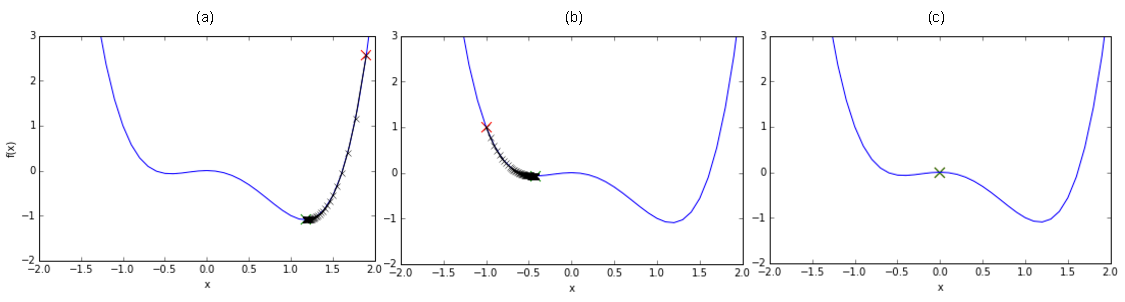
\includegraphics[scale=0.9]{polynomialdescent.pdf}
\caption{Visualization of gradient descent for three initial guesses, $x_0$, of the non-convex polynomial $f(x) = x^4 - x^3 -x^2$.  Initial guesses are: (a), 1.9; (b) -1.0; (c), 0.0.  The red $X$ marks the initial guess, the green $X$ marks the algorithm's final value, and the black $X$ represent sequential values produced by each gradient descent step. Plot (a) converges to the global minimum, while (b) converges to a local, non-global minimum.  Plot (c) remains at the initial guess, since $f'(x_0)=0$. Shown are results using: analytical gradients, $\eta = 0.02$, $\epsilon = 0.0004$.}
\label{poly}
\end{figure*}

Where in $p(\mathbf{x})$, $\mathbf{\Sigma}$ represents the covariance and $\boldsymbol{\mu}$ the mean.  Note also that the standard Gaussian has been multiplied by $-1$ (so that we can pose our optimization as a minimization) and scaled by $100$, which is just to help with making plotting more clear.

\begin{figure*}[!ht]
\centering
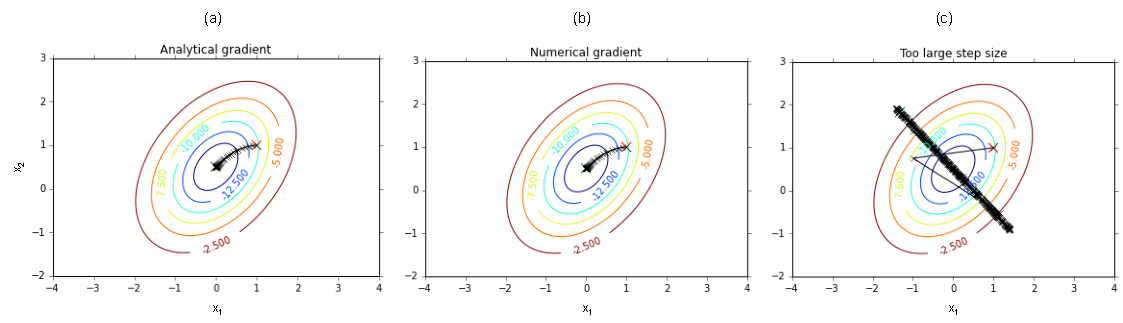
\includegraphics[scale=0.9]{negGaussianDescent.pdf}
\caption{Visualization of gradient descent for the negative bivariate Gaussian $p(x)$, plotted via contours.  The red $X$ marks the initial guess $x_0$, the green $X$ marks the algorithm's final value, and the black $X$ represent sequential values produced by each gradient descent step.  Plots (a) and (b) show a comparison of using the analytical vs. numerical gradients: note although the descent path looks similar, the number of function calls is an order of magnitude different.   Plot (c) shows the path of gradient descent when the step size is too large ($\eta = 0.2$). Unless otherwise noted, all plots used: $x_0 = (1.0,1.0)$, $\eta = 0.01$, $\epsilon = 0.0004$.}
\label{gauss}
\end{figure*}

The effects of initial guesses ($x_0$) and varying step size ($\eta$) are best explained via the plots.  For the non-convex polynomial, $f(x)$, the effect of the starting position can be seen from the three plots in Figure \ref{poly}.  Initial guesses $x_0 > 0$ will terminate at the global maximum of the function, whereas initial guesses $x_0 < 0$ get ``stuck'' at the local minimum in $\mathbb{R}^-$.  An initial guess of exactly a local maximum $x_0 = 0$ leads to the algorithm terminating still with $x_{final} = 0$ after only a handful of iterations, since initially $f'(x=0)=0$.  It is nice to note that local maxima can cause algorithm termination with poor initial guesses, but in practice adding randomization to initial guesses helps mitigate this problem.  The effect of the step size can be viewed by observing the counter plots for gradient descent on $p(\mathbf{x})$, the bivariate Gaussian.  In plots (a) and (b), the step size is sufficiently small and successful descent occurs to the global minimum.  In plot (c), however, the step size is sufficiently large such that the algorithm continually jumps ``back and forth'' over the minimum, and the algorithm terminates only due to the maximum number of function calls ($n_{max}=5000$ was used).  Increasing the convergence criterion increases the number of iterations required to converge.  In practice as long as the convergence criterion is significantly smaller than the basins of attraction for the local minima, there is little effect on the algorithm other than increasing the number of iterations before termination.

Numerical gradients were also implemented by calculating finite differences.  Note that for numerical gradients, the required amount of function evaluations increases by a factor of $2d$, where $d$ is the dimension of the input.  A comparison of results for analytical vs. numerical gradients is provided in the three tables below.  For all points tested, analytical and numerical gradients resulted in the same termination value, although analytical gradients were typically able to find this value in approximately 1/5th the function calls for the $1$-dimensional function, and 1/10th the function calls for the $2$-dimensional Gaussian.

The comparison of our gradient descent implementation with \url{scipy.optimize} is interesting for a couple of reasons.  For one, despite best efforts to tune step sizes and convergence criterions, there is no way that our optimizer can match the SciPy optimizer in terms of required function calls.  SciPy's default BFGS (Broyden-Fletcher-Goldfarb-Shanno) optimization method, which we used, provides a more sophisticated method of descent than our simple first-order finite differencing.  We did not provide any analytical gradients to the optimizer, and so it computed them numerically.  Comparing apples to apples, our numerical gradient descent required a factor of approximately 50 times more function calls to converge, and even our analytical gradient descent required 3-10 times more function calls.  Despite its fast convergence performance, however, the SciPy optimizer did behave oddly on two of our tested initial conditions for the non-convex polynomial $f(x)$.  As shown in the second table below (no, this was not a typo), the SciPy optimizer returned the non-global minimum when the initial guess was in the basin of the global minimum, and returned the global minimum when it was in the basin of the non-global minimum.  This suggests \url{min(gradDescent,spicy.optimize)} is the safest optimization algorithm for our tested results.





\textit{Number of function calls}

\begin{tabular}{|l|l|l|l|}
\hline
Function and & & &\\ Initial Guess, $x_0$ & Analytical & Numerical & Scipy \\ \hline
\textit{Non-convex} $f(x)$ & & &\\ \hline
$x_0 = 1.9$ & $130$ & $646$ & $24$\\\hline
$x_0 = -1.0$ & $312$ & $1556$ & $36$ \\ \hline
$x_0 = 0.0$ & $2$ & $6$ & $3$\\ \hline
\textit{Neg. Gaussian} $p(x)$ & & & \\ \hline
$x_0 = (1.0,1.0)$ & $177$ & $1603$ & $48$ \\ \hline
\end{tabular}

\textit{Minimum $x$}

\begin{tabular}{|l|l|l|l|}
\hline
Function and & & &\\ Initial Guess, $x_0$ & Analytical & Numerical & Scipy \\ \hline
\textit{Non-convex} $f(x)$ & & &\\ \hline
$x_0 = 1.9$ & $1.17$ & $1.17$ & $-0.43$\\\hline
$x_0 = -1.0$ & $-0.43$ & $-0.43$ & $1.17$ \\ \hline
$x_0 = 0.0$ & $0.0$ & $2.5e-13$ & $0$\\ \hline
\textit{Neg. Gaussian} $p(x)$ & & & \\ \hline
$x_0 = (1.0,1.0)$ & $(0,0.5)$ & $(0,0.5)$ & $(0,0.5)$ \\ \hline
\end{tabular}

\textit{Minimum function value}

\begin{tabular}{|l|l|l|l|}
\hline
Function and & & &\\ Initial Guess, $x_0$ & Analytical & Numerical & Scipy \\ \hline
\textit{Non-convex} $f(x)$ & & &\\ \hline
$x_0 = 1.9$ & $-1.10$ & $-1.10$ & $-0.07$\\\hline
$x_0 = -1.0$ & $-0.07$ & $-0.07$ & $-1.10$ \\ \hline
$x_0 = 0.0$ & $0.0$ & $-6.3e-26$ & $0$\\ \hline
\textit{Neg. Gaussian} $p(x)$ & & & \\ \hline
$x_0 = (1.0,1.0)$ & $-17.36$ & $-17.36$ & $-17.36$ \\ \hline
\end{tabular}



\section{Linear Basis Function Regression}
We implemented the linear basis function regression in python and were able to get good agreement of our plots and regression weights with those in Bishop. We omit these plots for brevity. The closed form solution to the linear least squares problem is convenient, however it requires inverting the matrix $\Phi^T \Phi$. An alternative to avoid this matrix inversion is to apply gradient descent to the sum of squared error (SSE) objective function given by $(\Phi w - y)^T(\Phi w - y)$. Differentiating the SSE with respect to $w$ gives a gradient of $2\Phi^T(\Phi^T w - y)$. We checked this analytical gradient against our numerical gradient implementation. Using $h = 1e-5$ in the central difference computation led to agreement between analytical and numerical gradient to with $1e-8$ for $M = 3$. Using this analytical gradient we can apply our gradient descent code from problem 1. Our code employs a fixed step size of $\eta$ and the termination criterion is as soon as $\epsilon_{n+1} = |SSE(w_n) - SSE(w_{n+1})| \leq \gamma $ where $\gamma$ is a tolerance parameter. Our initial parameter choices are $\eta = 0.05, \gamma = 1 \times 10^{-8}$. The initial guess is set to $w_0 = -w_{OLS}$ where $w_{OLS}$ are the true regression weights. For $M = 1$ gradient descent works quite well.

\begin{tabular}{|l|l|l|}
\hline
Solver & Function Calls & Weights \\ \hline
Gradient Descent & 113 & $(0.820, -1.267)$ \\ \hline
Scipy & 20 & $(0.820, -1.267)$ \\ \hline
OLS  & - & $(0.820, -1.267)$ \\ \hline
\end{tabular}
%

Our gradient descent method converges to essentially the same regression weights as the scipy.optimize.minimize method and the true OLS regression weights, albeit with an order of magnitude more function calls. This is to be expected as the SSE function is convex in $w$ and hence there is a unique global minimum which can be reached by ``following'' the gradient downhill. Changing the initial guess to all zeros produces very similar performance in terms of objective value and number of function calls. With $M=3$ however the performance of our solver changes dramatically however. In particular, if $w_{OLS}$ denote the true regression weights then

\begin{tabular}{|l|l|l|l|}
\hline
Solver & Function Calls & $|w - w_{OLS}|_2$ & $\eta$ \\ \hline
Grad. Desc. & $38,513$ & $0.14$ & $0.05$ \\ \hline
Grad. Desc. & $72, 657$ & $0.199$ & $0.025$ \\ \hline
Scipy & 114 & $4\times 10^{-5}$ & - \\ \hline
\end{tabular}
%
%

Thus increasing the dimension of the optimization problem from 2 to 4 exposes the weaknesses of our gradient descent method. In particular it uses about $300$ times more function calls. The reason is that as we approach the optimum the SSE function becomes very flat and hence the gradient $\nabla SSE$ becomes very small. Hence, in our update step $w_{n+1} = w_n - \eta*\nabla SSE(w_n)$ the amount we move, $\eta*\nabla SSE(w_n)$ is becoming arbitrarily small. In particular if we plot function value vs iterations (Figure \ref{grad-descent-iterations}) we see that the plot becomes very flat quite quickly. Thus for most of the iterations of the algorithm we aren't really decreasing the value of the objective very much. 

\begin{figure}[h]
\centering
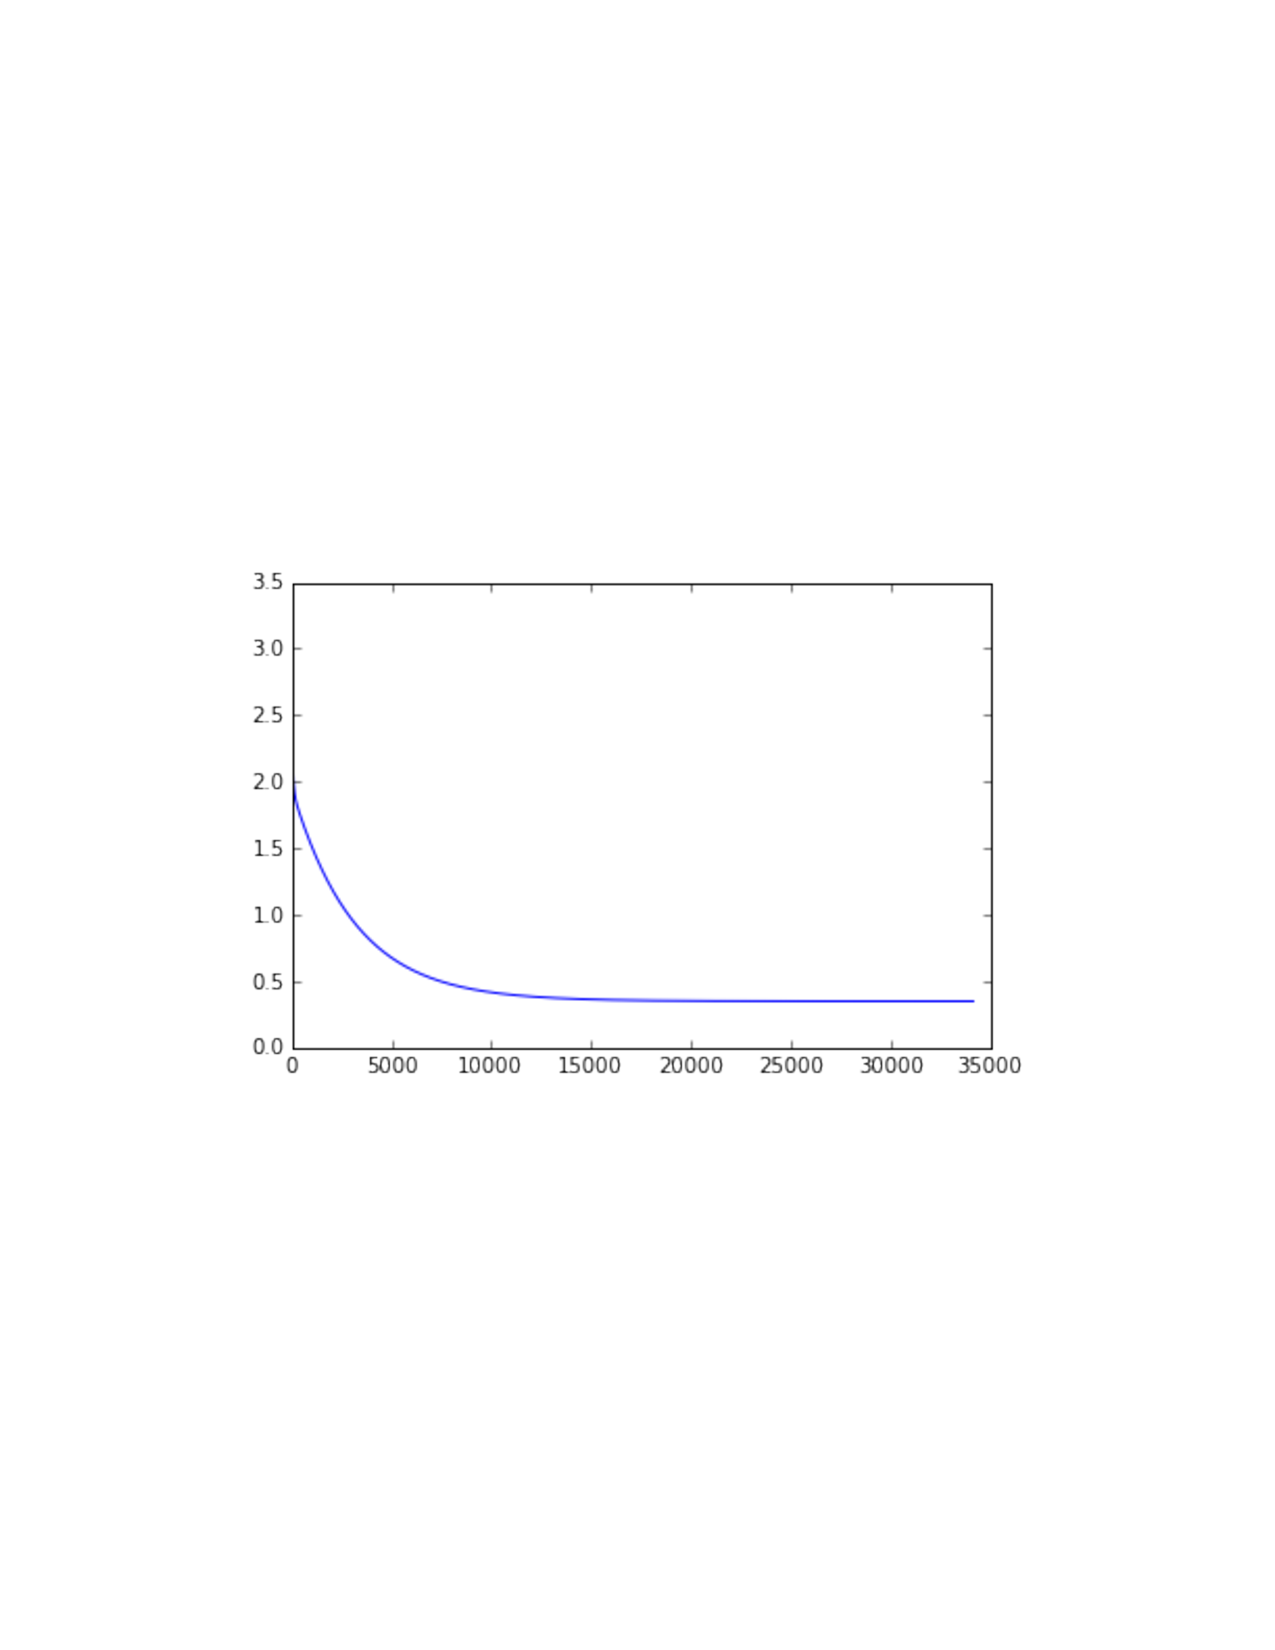
\includegraphics[width=0.4\textwidth]{lin-reg-fig-1}
\caption{Value of SSE at each iteration of our gradient descent algorithm, $\eta = 0.05$, $w_0 = 0$}
\label{grad-descent-iterations}
\end{figure}

This is a result of our update step not moving us enough when the gradient becomes small. Reducing $\eta$ to $0.025$ just exacerbates this problem. In this case we require more iterations and achieve worse fit of the regression weights. If we try increasing $\eta = 0.07$ however the opposite happens. We adjust $w_{n+1}$ by too much and end up jumping to the other side of the ``bowl'' representing the SSE. Hence we end up bouncing back between different sides of the bowl and the solution ends up exploding. The effect of the inital guess for $M = 3$ isn't too important. Using $\eta = 0.05$ and choosing initial guess to the origin results in the number of function calls decreasing to about $34,000$ and doesn't change the achieved accuracy of the solution. This makes sense because since we are optimizing a convex function we have no risk of getting stuck in local minima and thus independent of where we start we should be able to follow the gradient down to the minimum.

The results for $M = 9$ are very interesting as well. The value of $SSE(w_{OLS})$ is $1e-7$. If we set the initial guess for the scipy minimization to be $w_0 = 1.5*w_{OLS}$ then it achieves a minimum value of $0.09$ however if we set $w_0 = 0$ then the method only achieves $SSE = 0.314$. Our own gradient descent method behaves similarly. Thus in this case the performance of the gradient descent method is quite sensitive to the initial guess. A graphical illustration of the difference in the regression function can be seen in Figures \ref{m_9_grad_descent_good} and \ref{m_9_grad_descent_bad} and the difference in fit is quite striking. Thus the initial guess for gradient descent has a very large impact on the shape of the regression function for the $M = 9$ case.
%
\begin{figure}[h]
\centering
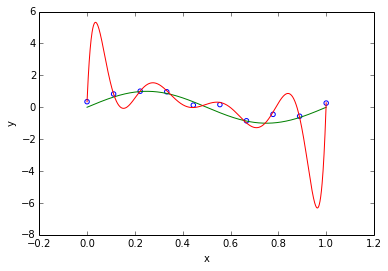
\includegraphics[width=0.4\textwidth]{m_9_grad_descent_good}
\caption{Gradient descent with $M = 9, w_0 = 1.5*w_{OLS}$. Blue are datapoints, green is true regression function, red is estimated regression function}
\label{m_9_grad_descent_good}
\end{figure}
\begin{figure}[h]
\centering
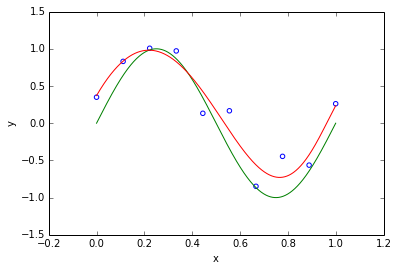
\includegraphics[width=0.4\textwidth]{m_9_grad_descent_bad}
\caption{Gradient descent with $M = 9, w_0 = 0*w_{OLS}$. Blue are datapoints, green is true regression function, red is estimated regression function}
\label{m_9_grad_descent_bad}
\end{figure}
%
%
I believe that this is because since we are considering large powers of $x$ the function is very flat near the minimum. Thus gradient descent methods have a hard time making progress towards the minimum since the function is locally very flat. 

If the basis functions were of the form $\phi_n(x)=\sin(2\pi n x)$ then we would expect a regression vector of the form $w = (1,0,0,...,0)$ since the data was actually generated from $\sin(2 \pi x)$ with Gaussian noise added. A potential disadvantage is that since the sin function is periodic you are imposing periodicity on your data. In particular $x $ and $x+1$ will map to the same value. In addition the set of functions $\mathcal{B} = \{\sin(2 \pi m x)\}_{m \in \mathbb{N}}$ aren't a basis for the space of functions. You need both $\sin$ and $\cos$ to form a basis. Thus there are functions, and hence datasets that are generated from such functions, that could not be well approximated by the basis $\mathcal{B}$.


%%%%%%%%%%%%%%%%%%%%%%%%%%%%%%%%%

\section{Ridge Regression}
As we saw in the previous section $M = 3$ provides a fairly good fit to the data. As can be seen in Figure \ref{ridge_m_3_lam_0-01} using $M = 3, \lambda = 0.01$ doesn't provide good performance.

\begin{figure}[h]
\centering
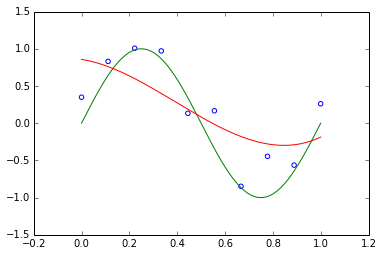
\includegraphics[width=0.4\textwidth]{m_3_lam_0-01}
\caption{Ridge regression with $M = 3, \lambda = 0.01$. $SSE = 1.54$. Blue are datapoints, green is true regression function, red is estimated regression function}
\label{ridge_m_3_lam_0-01}
\end{figure} 
In particular the $\lambda$ weight is too high and keeps the regression weights close to zero, which results in a relatively flat nearly linear fit. Reducing $\lambda $ to $0.001$ as in Figure \ref{ridge_m_3_lam_0-001} produces better results, as can be seen by comparing the SSE's since it doesn't penalize the weights $w$ as much for being far from zero.
%
\begin{figure}[h]
\centering
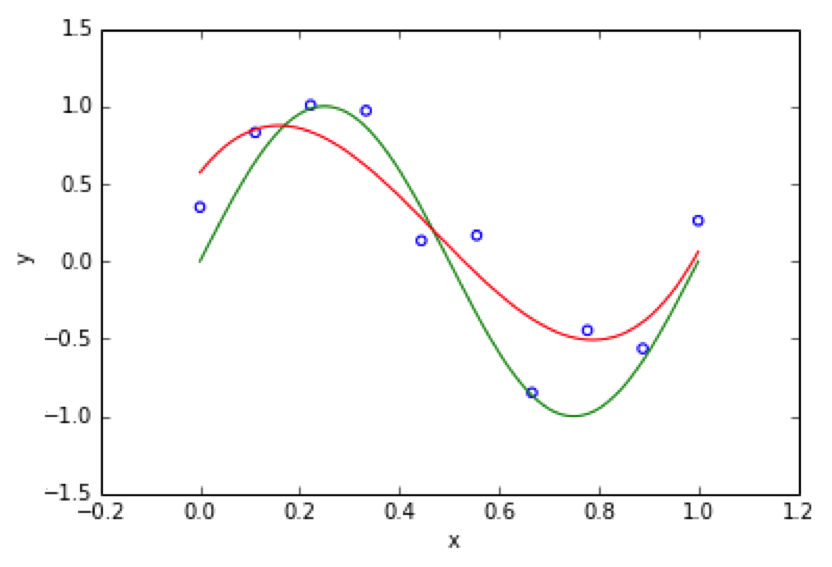
\includegraphics[width=0.4\textwidth]{m_3_lam_0-001}
\caption{Ridge regression with $M = 3, \lambda = 0.001$. $SSE = 0.588$. Blue are datapoints, green is true regression function, red is estimated regression function}
\label{ridge_m_3_lam_0-001}
\end{figure}
%
The interesting thing is that increasing $M$ while keeping $\lambda$ fixed doesn't adversely affect performance. In particular the prediction curve in red looks fairly similar even as we increase the number of features to $M = 9$ in Figure \ref{ridge_m_9_lam_0-001}. 
%
\begin{figure}[h]
\centering
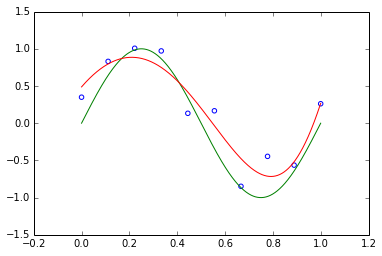
\includegraphics[width=0.4\textwidth]{m_9_lam_0-001}
\caption{Ridge regression with $M = 9, \lambda = 0.001$. $SSE = 0.418$. Blue are datapoints, green is true regression function, red is estimated regression function}
\label{ridge_m_9_lam_0-001}
\end{figure}
%
Thus the regularizer $\lambda$ helps us to avoid overfitting. In particular there is a very large difference between the fit between Figures \ref{ridge_m_9_lam_0-001} and \ref{m_9_grad_descent_good}.

For the train, validate and test datasets we perform the following model selection procedure. Given $(M,\lambda)$ we run ridge regression on the training dataset to find the regression weights $w(M,\lambda)$. Then we compute the SSE using weights $w(M,\lambda)$ on the validation dataset, denote this by $SSE_v(M,\lambda)$. We choose $(M,\lambda)$ to minimize $SSE_v(M,\lambda)$. In essence we are using the training set to choose the weights, and then using the validation set to optimize over the model, given by $(M,\lambda)$. For each $M$ we search over $\lambda \in [0,10]$ to minimize $SSE_v(M,\lambda)$. Then we can check how well our model is doing on the test dataset. Table \ref{model-selection} shows the results.

\begin{table}
\begin{tabular}{|l|l|l|l|l|}
\hline 
$M$ & $\lambda$ & SSE Train & SSE Validate & SSE Test \\ \hline
$1$ & $6.53$ & $18.36$ & $16.89$ & $16.89$ \\ \hline
$2$ & $1.89$ & $12.4$ & $8.92$ & $24.1$ \\ \hline
$3$ & $0.1$ & $9.84$ & $3.6$ & $23.3$ \\ \hline
$4$ & $0.854$ & $8.7$ & $0.98$ & $27.7$ \\ \hline
$5$ & $8.9$ & $10.3$ & $2.19$ & $36.5$ \\
\hline
\end{tabular}
\label{model-selection}
\caption{SSE for training, validation and test datasets for different $M$. The specified $\lambda$ minimizes SSE for validation set given that $M$.}
\end{table}
%
%
The result of the model selection is $M=4,\lambda=0.85$. However this is misleading result. Consider the plot of the three datasets and the prediction function in Figure \ref{m-4-model-selection}.
%
%
\begin{figure}[h]
\centering
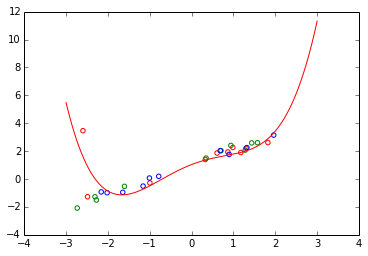
\includegraphics[width=0.4\textwidth]{m-4-model-selection}
\caption{Ridge regression with $M = 4, \lambda = 0.85$. Train datapoints are red, validation are blue, and test are green. Estimated regression function is in red.}
\label{m-4-model-selection}
\end{figure}
%
%
Visually the data look linear. However the one outlier in the training set is leading to bad fits for the $M = 1$ case as can be seen in Figure \ref{m-1-model-selection}.
%
\begin{figure}[h]
\centering
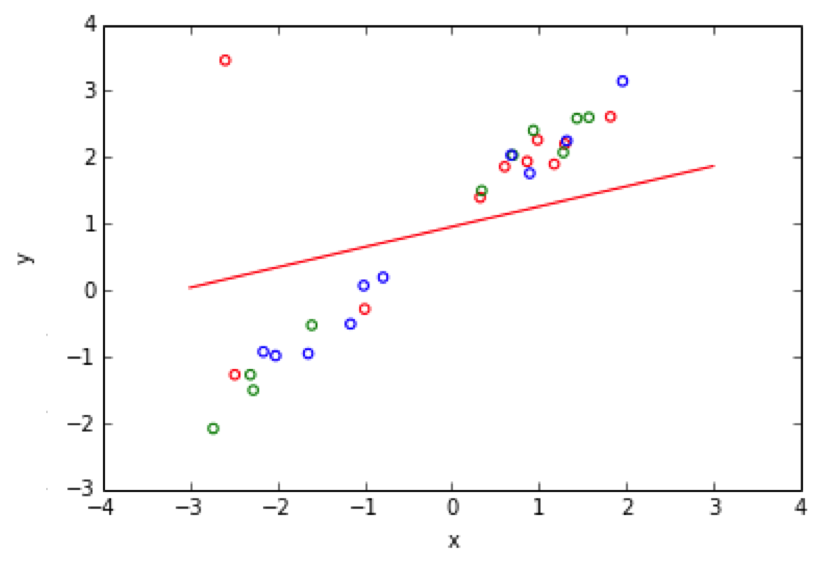
\includegraphics[width=0.4\textwidth]{m-1-model-selection}
\caption{Ridge regression with $M = 1, \lambda = 6.5$. Train datapoints are red, validation are blue, and test are green. Estimated regression function is in red.}
\label{m-1-model-selection}
\end{figure}
%
%
%
Hence when we perform our model selection procedure we end up choose $M = 4$ rather than $M = 1$ because this choice of $M$ allows us to roughly hit the outlier and the bulk of the validation data points. However since the test set extends to larger magnitude $x$ values, we have a terrible fit on the test dataset, even though we get a relatively good fit on the validation data. Thus the lesson is that in the presence of outliers model selection together with ridge regression can lead us to incorrect results.
%
%

For the blog feedback there is only one parameter to choose during model selection, namely $\lambda$ since the feature set $\Phi$ has already been specified for us. We ran ridge regression with a variety of $\lambda$ values and to compare performance. We saw that fairly large $\lambda$ around $3000$ were providing the best performance. Similar to the previous analysis we then performed a grid search over $\lambda$ to choose the best model. The results are shown in Figure \ref{blog-model-selection}. Note that the $\Phi$ matrix is not full rank since several of the features are identically zero for all observations.
%

%
%
%
\begin{figure}[h]
\centering
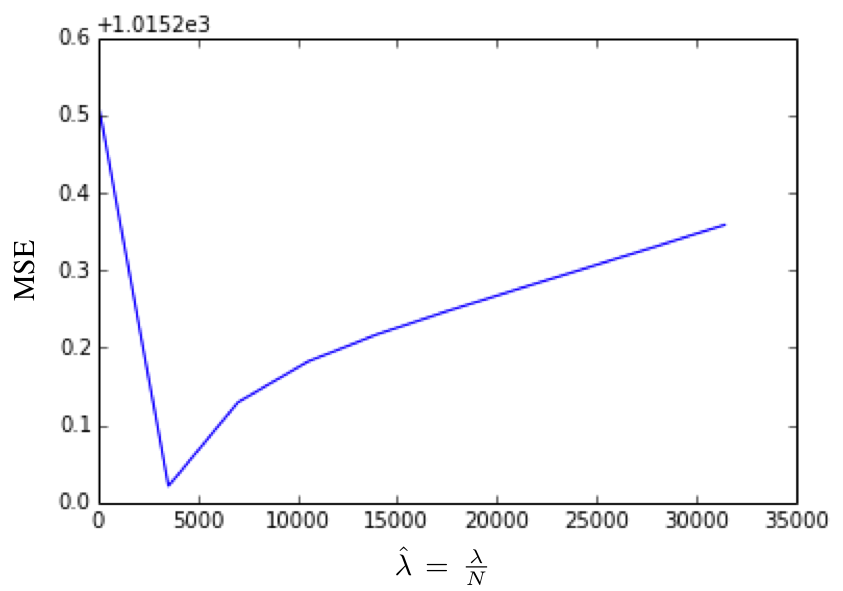
\includegraphics[width=0.4\textwidth]{blog-model-selection}
\caption{The x-axis is $\hat{\lambda} = \frac{\lambda}{N}$ plotted against the MSE of the validation set on the y-axis.}
\label{blog-model-selection}
\end{figure}
%
Interestingly the plot is very flat. In other words the MSE of the validation set isn't very sensitive to the parameter $\lambda$.  So the choice of regularize $\lambda$ is not having too much of an effect on the MSE of the validation data. In particular it seems that the fit of the model is much less dependent on $\lambda$ than in the curvefitting example.  The plot of $\lambda$ against the MSE of the test set looks quite different however. It decreases fairly continuously as $\lambda$ increases, see Figure \ref{blog-model-select-test}.
 %
 %
\begin{figure}[h]
\centering
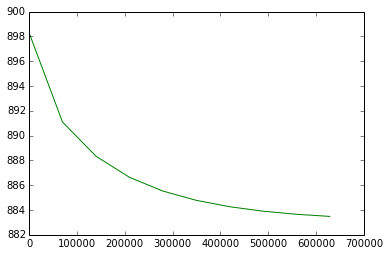
\includegraphics[width=0.4\textwidth]{blog-model-select-test}
\caption{The x-axis is $\hat{\lambda} = \frac{\lambda}{N}$ plotted against the MSE of the test set on the y-axis.}
\label{blog-model-select-test}
\end{figure}
 %
 %
Looking at the actual regression weights $w$ shows for $\lambda = 3000$ they are less than $1.5$ in absolute value.

%
%

Now we compare the results to performing feature rescaling using the interval method. Namely for each feature $\phi_i(x)$ we rescale it to 
%
%
%
\begin{equation*}
\tilde{\phi}(x) = \frac{\phi_i(x) - \min_{x'}\phi_i(x')}{\max_{x'}\phi_i(x') - \min_{x'}\phi_i(x)}
\end{equation*}
 %
 %
 where max and min are over the observed values of that feature in the dataset. Some care had to be taken because some features were identically zero. The rescaling implies that the new features satisfy $\tilde{\phi}(x) \in [0,1]$.  Repeating the above analysis with the rescaled features gives
 %
 %
 Now we see that the MSE of the validation set is much more responsive to varying $\lambda$. However, we again notice that the plots of MSE look very different for the validation and test sets. This is somewhat surprising since neither of these datasets was used to train the regression weights. Interestingly looking at the regression weights after provides an interesting insight. Let $w$ be the regression weights with $\lambda = 350$. Then interestingly we see that most of the values are near zero and with a few notable exceptions see Figure \ref{reg-weights-lam-350-normalize-true}. Thus this shows that a small number of features are responsible for predicting the number of comments.
%
 \begin{figure}[h]
\centering
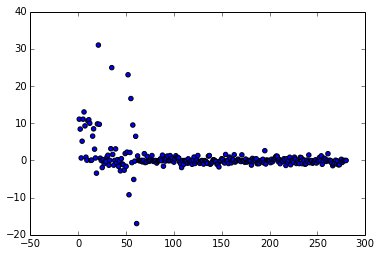
\includegraphics[width=0.5\textwidth]{reg-weights-lam-350-normalize-true}
\caption{A plot of the regression weights vs their index. Weights gotten using the feature rescaling with $\lambda = 350$. }
\label{reg-weights-lam-350-normalize-true}
\end{figure}
%
%
Ultimately we achieved a smaller MSE on the test set when we didn't rescale the features. However, the insight we get from running the ridge regression with the rescaled features is that, as can be seen in Figure \ref{reg-weights-lam-350-normalize-true}, a few of the features contain most of the predictive power for the number of comments. The other thing that feature rescaling affects is the role of the regularization term $\lambda ||w||_2^2$. In particular rescaling the features also to some extent should rescale the weights $w$. Since the $\lambda$ term affects all weights equally in the regularization term, it proportionally now drives down the weights on the ``important'' features from Figure \ref{reg-weights-lam-350-normalize-true} more than it drives down those same weights in the unregularized dataset. Ultimately it is difficult to draw too many more specific conclusions since it is challenging to visualize data with $280$ features.



\section{Implement Gradient Descent}
A general-purpose gradient descent library was created which provides for specification of $x_0$ (the initial guess), $\eta$ (the step size), and $\epsilon$ (the convergence threshold: if two consecutive steps differ by less than this value, the algorithm terminates).



% In the unusual situation where you want a paper to appear in the
% references without citing it in the main text, use \nocite
\nocite{langley00}

\bibliography{example_paper}
\bibliographystyle{icml2015}

\end{document} 


% This document was modified from the file originally made available by
% Pat Langley and Andrea Danyluk for ICML-2K. This version was
% created by Lise Getoor and Tobias Scheffer, it was slightly modified  
% from the 2010 version by Thorsten Joachims & Johannes Fuernkranz, 
% slightly modified from the 2009 version by Kiri Wagstaff and 
% Sam Roweis's 2008 version, which is slightly modified from 
% Prasad Tadepalli's 2007 version which is a lightly 
% changed version of the previous year's version by Andrew Moore, 
% which was in turn edited from those of Kristian Kersting and 
% Codrina Lauth. Alex Smola contributed to the algorithmic style files.  
